\documentclass[convert = false, tikz]{standalone}
\usepackage[utf8]{inputenc}
\usepackage{tikz}
\usetikzlibrary{automata, positioning, arrows, shapes.geometric}

\usepackage{../../../../style_automata}

% arara: pdflatex
% arara: latexmk: { clean: partial }
\begin{document}
    \tikzset{
    node distance=2cm, % specifies the minimum distance between two nodes.
    }
    \scalebox{0.8}{
    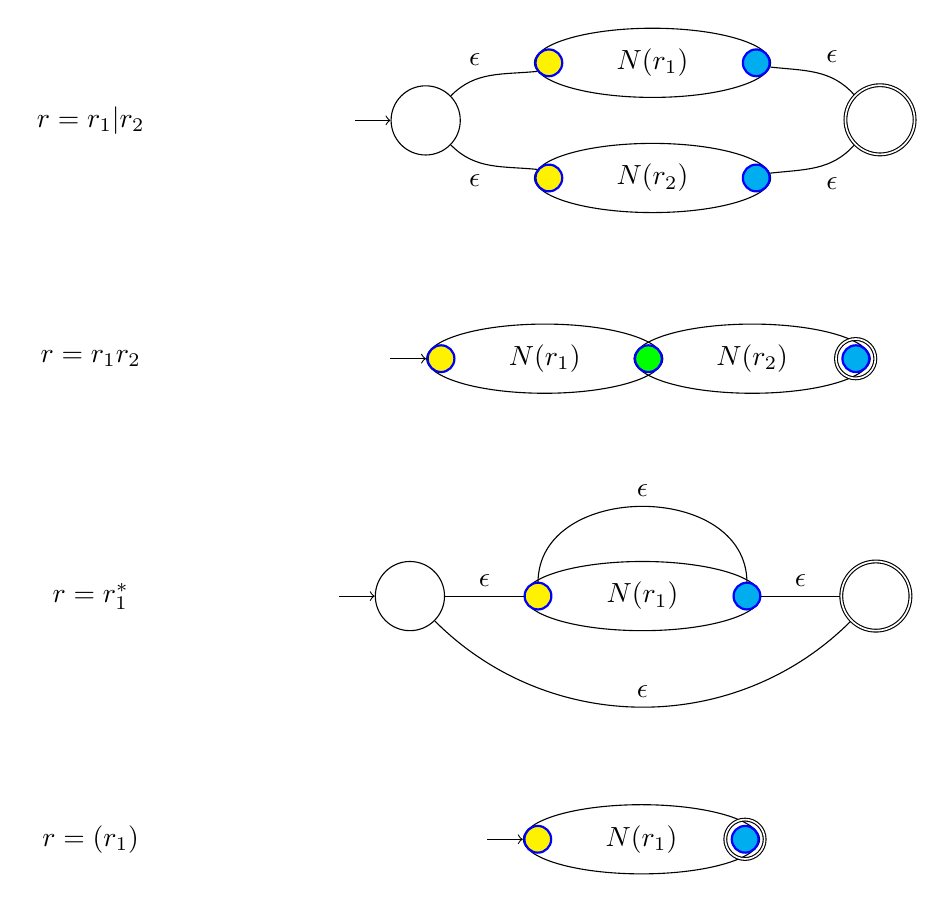
\begin{tikzpicture}
        \path node(l0){$r = r_1 | r_2$};
        \path node(l1)[below=2.5cm of l0]{$r = r_1 r_2$};
        \path node(l2)[below=2.5cm of l1]{$r = r_1^*$};
        \path node(l3)[below=2.5cm of l2]{$r = (r_1)$};

        % r = r_1 | r_2
        \node[state, initial, initial text=, right=3cm of l0] (s0) {};
        \node[state, ellipse, minimum width=3cm, above right=0.1cm and 1.5cm of s0]  (s01) {$N(r_1)$};
        \node[state, ellipse, minimum width=3cm, below right=0.1cm and 1.5cm of s0] (s02) {$N(r_2)$};
        \node[state, accepting, above right=0.1cm and 1.5cm of s02] (s03) {};
        
        \draw (s0) edge[above left, bend left, in=170] node{$\epsilon$} (s01);
        \draw (s0) edge[below left, bend right, in=-170] node{$\epsilon$} (s02);
        \draw (s01) edge[above right, bend left, out=12] node{$\epsilon$} (s03);
        \draw (s02) edge[below right, bend right, out=-12] node{$\epsilon$} (s03);
        
        \node[circle,fill,draw=blue,thick,inner sep=1.2mm,outer sep=1mm,fill=yellow, left=-0.46cm of s01] (c01) {};
        \node[circle,fill,draw=blue,thick,inner sep=1.2mm,outer sep=1mm,fill=cyan, right=-0.46cm of s01] (c02) {};
        \node[circle,fill,draw=blue,thick,inner sep=1.2mm,outer sep=1mm,fill=yellow, left=-0.46cm of s02] (c03) {};
        \node[circle,fill,draw=blue,thick,inner sep=1.2mm,outer sep=1mm,fill=cyan, right=-0.46cm of s02] (c04) {};


        % r = r_1 r_2
        \node[state, ellipse, minimum width=3cm, initial, initial text=, right=3.5cm of l1] (s1) {$N(r_1)$};
        \node[state, ellipse, minimum width=3cm, right=-0.38cm of s1] (s11) {$N(r_2)$};
        \node[state, accepting, minimum size=0.5cm, right=-0.46cm of s11] (s12) {};
        
        \node[circle,fill,draw=blue,thick,inner sep=1.2mm,outer sep=1mm,fill=yellow, left=-0.46cm of s1] (c11) {};
        \node[circle,fill,draw=blue,thick,inner sep=1.2mm,outer sep=1mm,fill=green, right=-0.46cm of s1] (c12) {};
        \node[circle,fill,draw=blue,thick,inner sep=1.2mm,outer sep=1mm,fill=cyan, right=-0.46cm of s11] (c12) {};
        
        
        % r = r_1^*
        \node[state, initial, initial text=, right=3cm of l2] (s2) {};
        \node[state, ellipse, minimum width=3cm, right=1cm of s2] (s21) {$N(r_1)$};
        \node[state, accepting, right=1cm of s21] (s22) {};
        
        \node[circle,fill,draw=blue,thick,inner sep=1.2mm,outer sep=0mm,fill=yellow, left=-0.35cm of s21] (c21) {};
        \node[circle,fill,draw=blue,thick,inner sep=1.2mm,outer sep=0mm,fill=cyan, right=-0.35cm of s21] (c22) {};
        
        \draw (s2) edge[above] node{$\epsilon$} (s21);
        \draw (s21) edge[above] node{$\epsilon$} (s22);
        \draw (s2) edge[above, bend right, out=-45, in=-135] node{$\epsilon$} (s22);
        \draw (c22) edge[above, bend right, out=-90, in=-90, looseness=1.25] node{$\epsilon$} (c21);
        
        % r = (r_1)
        \node[state, ellipse, minimum width=3cm, initial, initial text=, right=4.75cm of l3] (s3) {$N(r_1)$};
        \node[state, accepting, minimum size=0.5cm, right=-0.46cm of s3] (s31) {};
        
        \node[circle,fill,draw=blue,thick,inner sep=1.2mm,outer sep=1mm,fill=yellow, left=-0.46cm of s3] (c31) {};
        \node[circle,fill,draw=blue,thick,inner sep=1.2mm,outer sep=1mm,fill=cyan, right=-0.46cm of s3] (c32) {};

    \end{tikzpicture}
    }
\end{document}